% !TEX root = ./informe.tex

\section{Introducción}

Un \textit{clique} en un grafo $G$ es un subconjunto de vértices que induce en $G$ un subgrafo completo. La \textit{frontera} de un subconjunto de vértices $S$ es el conjunto de vértices con un extremo en $S$ y otro en $G \setminus S$. El presente informe trata sobre el problema de encontrar un clique que maximice la cardinalidad de su frontera en un grafo determinado. \\

La palabra `clique' proviene de sociologia, en donde representa un grupo unido de individuos con intereses en común. Modelando redes sociales con grafos, la definición formal de clique que acabamos de realizar hasta cierto punto coincide con esta noción. Esto ocurre porque el hecho de que un grupo de personas en una red induzca un subgrafo completo implica que todas las personas están conectadas entre sí. Una observación razonable es que adyacencia total dos a dos puede ser una condicción demasiado restrictiva en un modelo estandar de relaciones personales. Sin embargo, hay formas de sortear estos problemas, como utilizar la definición de \textit{n-cliques} (Luce 1950, Alba 1973), que grosso modo, es una manera de relajar las adyacencias dentro de un grafo con el objetivo de admitir cliques que no calificarian con la definición estricta. De cualquier forma, lo que queremos mostrar es que la noción de clique se corresponde bien con la definición informal sobre redes sociales. \\

La utilidad de calcular cliques y resolver los problemas asociados a estos tiene su lugar en cierto ámbitos de la ciencia. Como dijimos en la parrafo anterior, el ejemplo más claro es que permiten obtener información acerca de las dinámicas dentro de una red social. Sin embargo, no es el único uso que se le puede dar. También pueden utilizarse en el contexto de la química, por ejemplo para detectar similaridades no triviales entre las estructuras de dos proteinas distintas \cite{proteins}. Pensando en el complemento de un grafo, también pueden ayudarnos a encontrar conjuntos de vértices independientes. Por ende, es de interés poder calcular cliques de manera computacionalmente eficiente. \todo{'tra ve' `calcular cliques'} \\

Lidiando con redes sociales con mucha información, podemos utilizar los cliques para presentar la información de forma más compacta y más representativa, lidiando con grupos en vez de individuos (que en un contexto social tienen más repercusión). \\

\begin{center}
	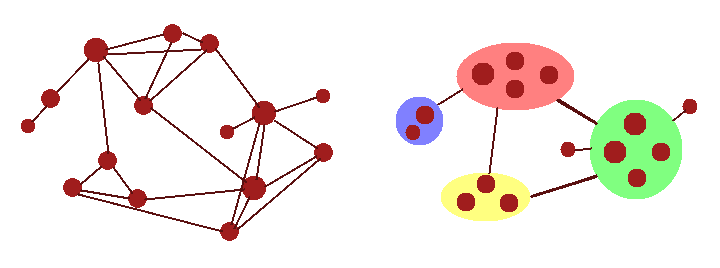
\includegraphics[scale=0.9]{imgs/example.png}
	\textit{Alalalala}
\end{center}

Como podemos ver, esto nos permite identificar mejor las dinámicas que tiene una red, y qué grupos tienen más influencia que otros.